\chapter{DESENVOLVIMENTO}

\section{Circuito Ceifador série com fonte}

Circuitos ceifadores possuem como objetivo, a realização de cortes no sinal de determinados períodos quando o circuito estiver polarizado inversamente. O circuito da imagem \ref{fig:ImagemSlide01} representa um sinal de entrada Vi, e o circuito ceifador com uma fonte em série que será utilizado posteriormente em simulação.

\begin{figure}[H]
    \centering
    \fbox{
        \parbox{0.975\textwidth}{
            \centering
            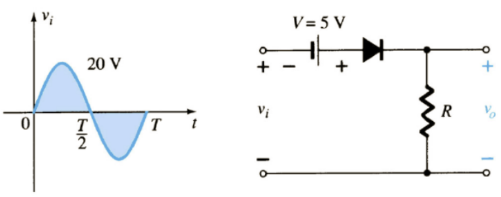
\includegraphics[width=0.975\textwidth]{images/imagem_slide_01.png}
        }}
    \caption{Circuito ceifador série com fonte}
    \vspace{-0.3cm}
    \label{fig:ImagemSlide01}
\end{figure}

\begin{figure}[H]
    \centering
    \fbox{
        \parbox{0.975\textwidth}{
            \centering
            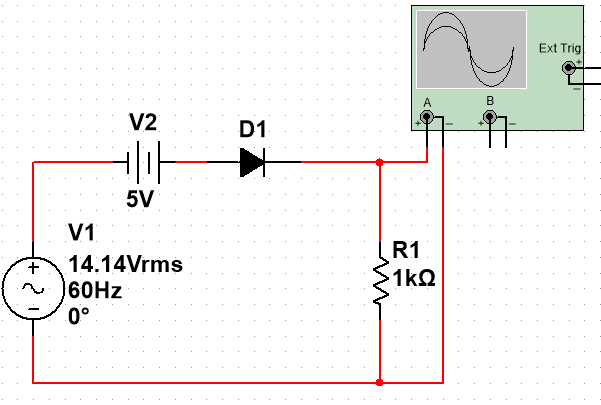
\includegraphics[width=0.975\textwidth]{images/simulacoes/circuito01.png}
        }}
    \caption{Simulação: Circuito ceifador série com fonte}
    \vspace{-0.3cm}
    \label{fig:SimulacaoCircuito01}
\end{figure}

\begin{figure}[H]
    \centering
    \fbox{
        \parbox{0.975\textwidth}{
            \centering
            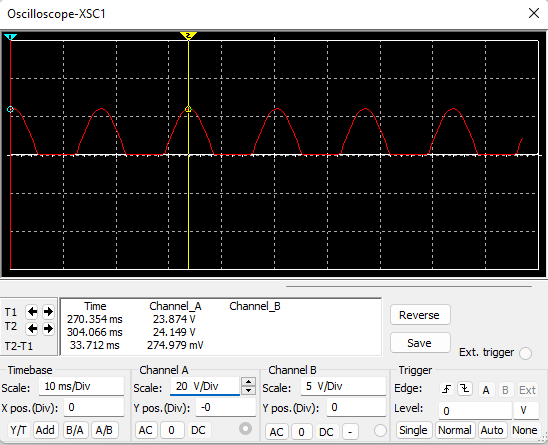
\includegraphics[width=0.975\textwidth]{images/simulacoes/osciloscopio_circuito01.png}
        }}
    \caption{Osciloscópio: Circuito ceifador série com fonte}
    \vspace{-0.3cm}
    \label{fig:OsciloscopioCircuito01}
\end{figure}

Através da imagem \ref{fig:OsciloscopioCircuito01}, podemos observar que o valor de vo de saída do circuito possui um pico de tensão de 24.065V. O valor de tensão teórico é calculado levando-se em consideração um diodo ideal, na qual não representa queda de tensão. Sendo assim, a tensão de pico do circuito será o valor somado da tensão da fonte de corrente alternada com a fonte de tensão de corrente contínua: \[20 + 5 = 25v\]

Com a tabela \ref{tab:Comparacao1Circuito} podemos comparar os resultados obtidos por simulação com os resultados obtidos por cálculo, na qual comprovam que os cálculos estavam corretos, com uma pequena diferença devido a aproximação.

\begin{quadro}[H]
    \centering
    \caption{Comparação entre os resultados obtidos por simulação e os resultados obtidos por cálculo do circuito 02}
    \begin{tabular}{|C{0.34\textwidth}|C{0.19\textwidth}|C{0.19\textwidth}|C{0.19\textwidth}|C{0.19\textwidth}|}
        \hline
        \rowcolor[HTML]{C0C0C0}
        \textbf{Modelo\textbackslash{}Variáveis} & \textbf{Vo} \\
        \hline
        Calculado & 25V \\
        \hline
        Simulado & 24.149V \\
        \hline
    \end{tabular}
    \vspace{-0.6cm}
    \label{tab:Comparacao1Circuito}
\end{quadro}

\section{Circuito com a fonte de tensão invertida}

No circuito da imagem \ref{fig:ImagemSlide02}, podemos observar que a fonte de tensão de corrente contínua está invertida, ou seja, sua polarização está inversa.

\begin{figure}[H]
    \centering
    \fbox{
        \parbox{0.975\textwidth}{
            \centering
            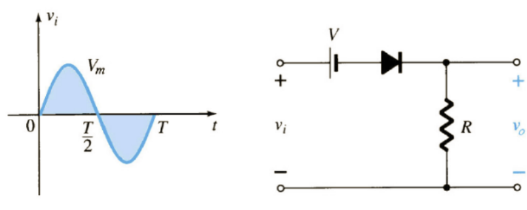
\includegraphics[width=0.975\textwidth]{images/imagem_slide_02.png}
        }}
    \caption{Circuito ceifador série com fonte invertida}
    \vspace{-0.3cm}
    \label{fig:ImagemSlide02}
\end{figure}

\begin{figure}[H]
    \centering
    \fbox{
        \parbox{0.975\textwidth}{
            \centering
            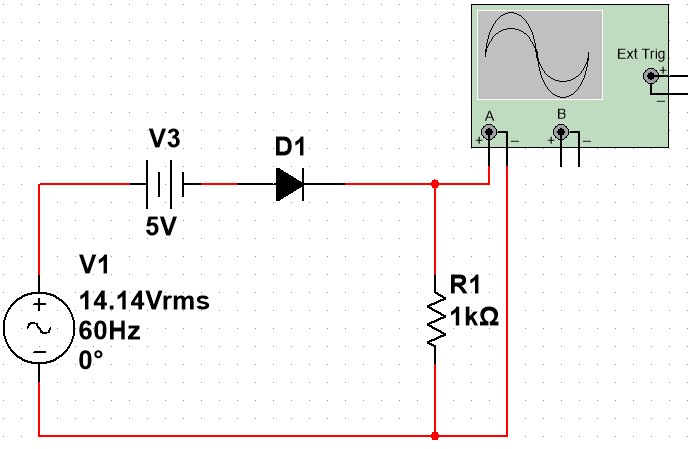
\includegraphics[width=0.975\textwidth]{images/simulacoes/circuito02.png}
        }}
    \caption{Simulação: Circuito ceifador série com fonte invertida}
    \vspace{-0.3cm}
    \label{fig:SimulacaoCircuito02}
\end{figure}

\begin{figure}[H]
    \centering
    \fbox{
        \parbox{0.975\textwidth}{
            \centering
            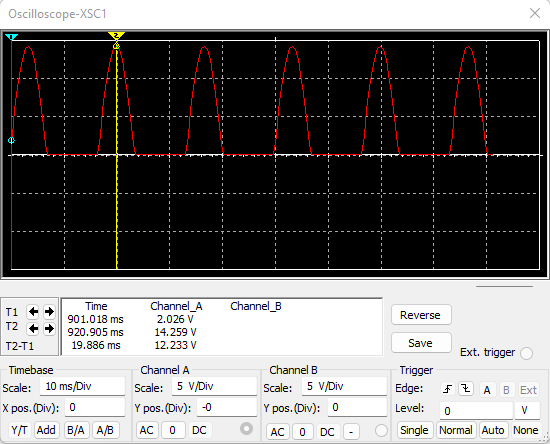
\includegraphics[width=0.975\textwidth]{images/simulacoes/osciloscopio_circuito02.png}
        }}
    \caption{Osciloscópio: Circuito ceifador série com fonte}
    \vspace{-0.3cm}
    \label{fig:OsciloscopioCircuito02}
\end{figure}

Podemos observar através da imagem \ref{fig:OsciloscopioCircuito02}, que o pico está em 14.259V, e o tempo que o sinal fica com o nível de tensão em 0v é maior do que o tempo em que ocorre a subida de onda; No semiciclo tem uma fonte de tensão de corrente contínua e invertida, a polarização do diodo é invertida até o momento em que a fonte de tensão de corrente alternada atinja o valor da fonte de tensão de corrente contínua, então a partir deste momento o diodo começa a ser polarizado.

Com a tabela \ref{tab:Comparacao2Circuito} podemos comparar os resultados obtidos por simulação com os resultados obtidos por cálculo, na qual comprovam que os cálculos estavam corretos, com uma pequena diferença devido a aproximação.

\begin{quadro}[H]
    \centering
    \caption{Comparação entre os resultados obtidos por simulação e os resultados obtidos por cálculo do circuito 02}
    \begin{tabular}{|C{0.34\textwidth}|C{0.19\textwidth}|C{0.19\textwidth}|C{0.19\textwidth}|C{0.19\textwidth}|}
        \hline
        \rowcolor[HTML]{C0C0C0}
        \textbf{Modelo\textbackslash{}Variáveis} & \textbf{Vo} \\
        \hline
        Teórico & 15V \\
        \hline
        Simulado & 14.259V \\
        \hline
    \end{tabular}
    \vspace{-0.6cm}
    \label{tab:Comparacao2Circuito}
\end{quadro}

\section{Ceifador paralelo com fonte}

Em um circuito ceifador paralelo com fonte, seu objetivo é cortar o sinal durante o semicírculo positivo da fonte de tensão. O circuito da imagem \ref{fig:ImagemSlide03} é um circuito ceifador paralelo com fonte.

\begin{figure}[H]
    \centering
    \fbox{
        \parbox{0.975\textwidth}{
            \centering
            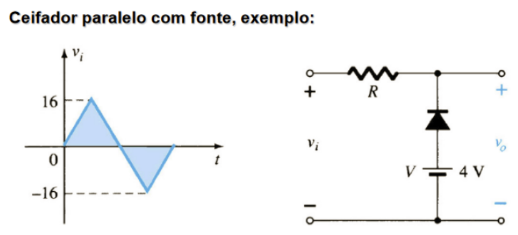
\includegraphics[width=0.975\textwidth]{images/imagem_slide_03.png}
        }}
    \caption{Circuito ceifador paralelo com fonte}
    \vspace{-0.3cm}
    \label{fig:ImagemSlide03}
\end{figure}

\begin{figure}[H]
    \centering
    \fbox{
        \parbox{0.975\textwidth}{
            \centering
            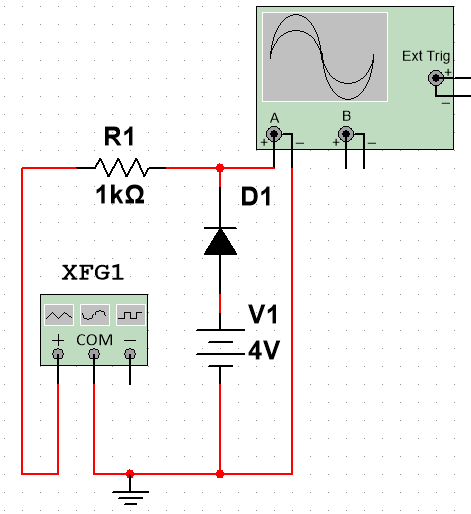
\includegraphics[width=0.975\textwidth]{images/simulacoes/circuito03.png}
        }}
    \caption{Simulação: Circuito ceifador paralelo com fonte}
    \vspace{-0.3cm}
    \label{fig:SimulacaoCircuito03}
\end{figure}

\begin{figure}[H]
    \centering
    \fbox{
        \parbox{0.975\textwidth}{
            \centering
            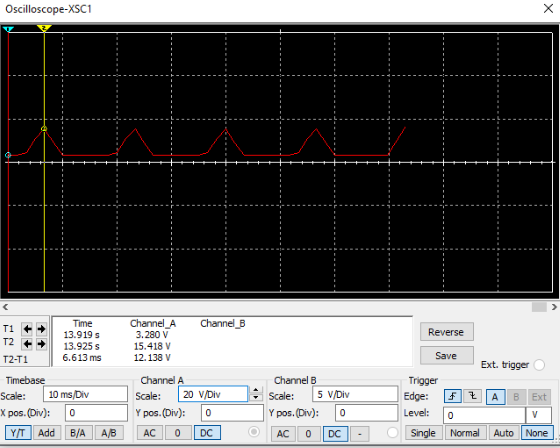
\includegraphics[width=0.975\textwidth]{images/simulacoes/osciloscopio_circuito03.png}
        }}
    \caption{Osciloscópio: Circuito ceifador série com fonte}
    \vspace{-0.3cm}
    \label{fig:OsciloscopioCircuito03}
\end{figure}

Pelo circuito simulado da imagem \ref{fig:SimulacaoCircuito03}, podemos analisar que inicialmente, a tensão DC polariza o diodo diretamente, porém, após o gerador de função atingir o nível de tensão maior do que o da fonte V1, o diodo é polarizado inversamente, e o sinal de saída visto é somente o sinal do gerador de função, como mostrado pela imagem \ref{fig:SimulacaoCircuito03}. 

Verificando o pico de sinal de saída de 15.418V, é possível entender que ele representa o período em que o gerador de função está polarizando o diodo inversamente, Pode-se observar que o sinal também já é iniciado com o valor de tensão maior que zero, pelo fato de o diodo já se iniciar polarizado diretamente pela fonte de 4V.

\section{Circuito Ceifador}

\begin{figure}[H]
    \centering
    \fbox{
        \parbox{0.975\textwidth}{
            \centering
            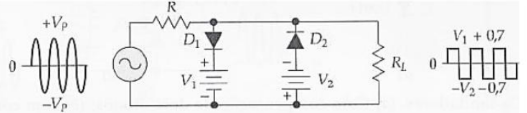
\includegraphics[width=0.975\textwidth]{images/imagem_slide_04.png}
        }}
    \caption{Circuito ceifador}
    \vspace{-0.3cm}
    \label{fig:ImagemSlide04}
\end{figure}

\begin{figure}[H]
    \centering
    \fbox{
        \parbox{0.975\textwidth}{
            \centering
            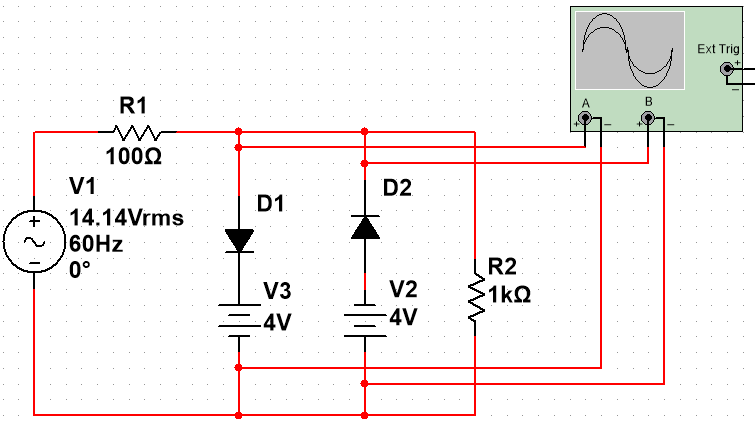
\includegraphics[width=0.975\textwidth]{images/simulacoes/circuito04.png}
        }}
    \caption{Simulação: Circuito ceifador}
    \vspace{-0.3cm}
    \label{fig:SimulacaoCircuito04}
\end{figure}

\begin{figure}[H]
    \centering
    \fbox{
        \parbox{0.975\textwidth}{
            \centering
            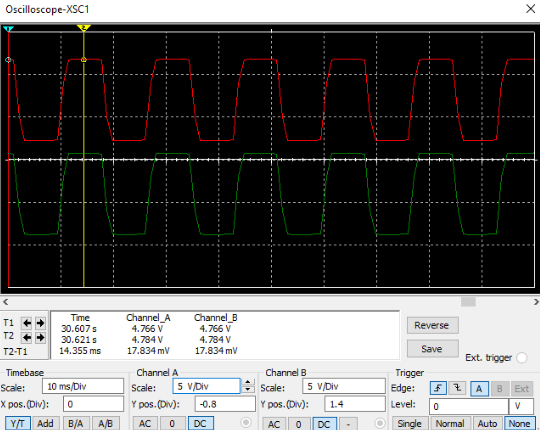
\includegraphics[width=0.975\textwidth]{images/simulacoes/osciloscopio_circuito04.png}
        }}
    \caption{Osciloscópio: Circuito ceifador}
    \vspace{-0.3cm}
    \label{fig:OsciloscopioCircuito04}
\end{figure}

O que podemos observar neste circuito, é que quando o D1 for polarizado, a tensão aplicada sobre a carga será apenas o V3. Porém, quando o D2 for polarizado, então a tensão sobre a carga será a de V2. Sendo assim, podemos analisar esta saída através da forma de onda gerada pelo osciloscópio da imagem \ref{fig:OsciloscopioCircuito04}, na qual possui a entrada máxima de V1 + 0.7V (Do diodo), e a mínima em -4V - 0.7V (Do diodo), pois a fonte está invertida..

\section{Circuito Grampeador}

O circuito grampeador tem por finalidade levar um sinal de entrada para a saída, abaixo ou acima de determinado nível, dependendo ou não se o mesmo for polarizado. O circuito grampeador é mostrado na imagem \ref{fig:ImagemSlide05}.

\begin{figure}[H]
    \centering
    \fbox{
        \parbox{0.975\textwidth}{
            \centering
            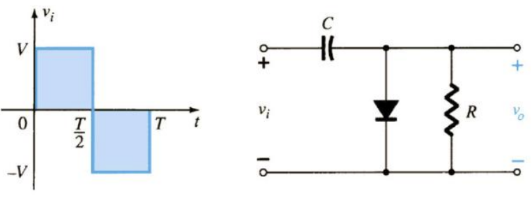
\includegraphics[width=0.975\textwidth]{images/imagem_slide_05.png}
        }}
    \caption{Circuito grampeador}
    \vspace{-0.3cm}
    \label{fig:ImagemSlide05}
\end{figure}

\begin{figure}[H]
    \centering
    \fbox{
        \parbox{0.975\textwidth}{
            \centering
            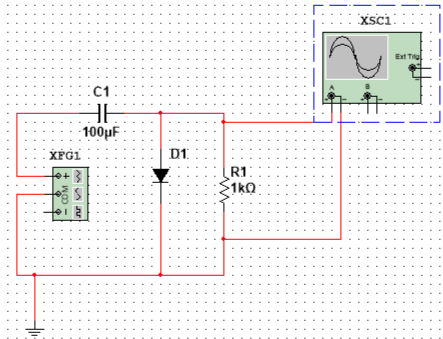
\includegraphics[width=0.975\textwidth]{images/simulacoes/circuito05.png}
        }}
    \caption{Simulação: Circuito grampeador}
    \vspace{-0.3cm}
    \label{fig:SimulacaoCircuito05}
\end{figure}

\begin{figure}[H]
    \centering
    \fbox{
        \parbox{0.975\textwidth}{
            \centering
            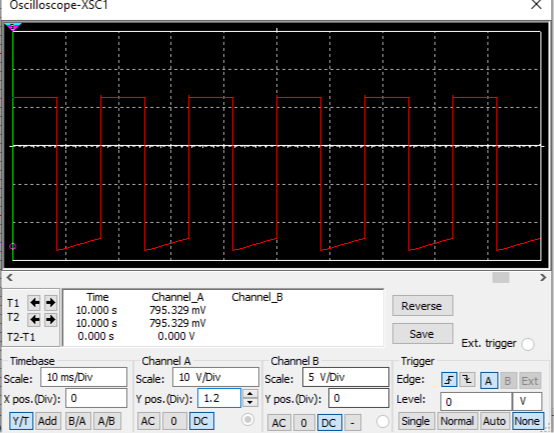
\includegraphics[width=0.975\textwidth]{images/simulacoes/osciloscopio_circuito05.png}
        }}
    \caption{Osciloscópio: Circuito grampeador}
    \vspace{-0.3cm}
    \label{fig:OsciloscopioCircuito05}
\end{figure}

Pode-se perceber que durante o semiciclo positivo da tensão de entrada, o diodo está polarizado diretamente, sendo assim, a tensão observada é de 0V, considerando o modelo de diodo ideal, o capacitor se carrega, e durante o período negativo da fonte, o diodo está polarizado inversamente, e a tensão observada sobre aquele ponto será a tensão da fonte somado a carga acumulada no capacitor. Como ainda existe um circuito fechado, esse capacitor se descarrega com o tempo, e então para que não ocorra essa descarga, é necessário uma frequência no mínimo 10x maior, na qual irá fazer com o que o capacitor seja carregado antes de o mesmo começar a se descarregar.

\section{Circuito grampeador com fonte em série}

\begin{figure}[H]
    \centering
    \fbox{
        \parbox{0.975\textwidth}{
            \centering
            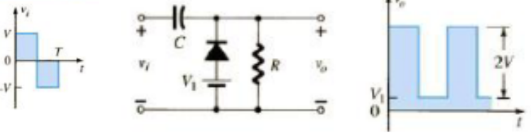
\includegraphics[width=0.975\textwidth]{images/imagem_slide_06.png}
        }}
    \caption{Circuito grampeador com fonte em série}
    \vspace{-0.3cm}
    \label{fig:ImagemSlide06}
\end{figure}

\begin{figure}[H]
    \centering
    \fbox{
        \parbox{0.975\textwidth}{
            \centering
            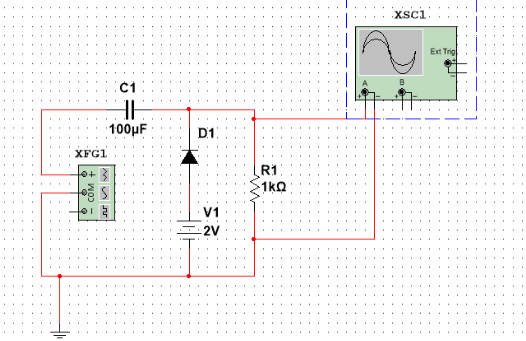
\includegraphics[width=0.975\textwidth]{images/simulacoes/circuito06.png}
        }}
    \caption{Simulação: Circuito grampeador com fonte em série}
    \vspace{-0.3cm}
    \label{fig:SimulacaoCircuito06}
\end{figure}

\begin{figure}[H]
    \centering
    \fbox{
        \parbox{0.975\textwidth}{
            \centering
            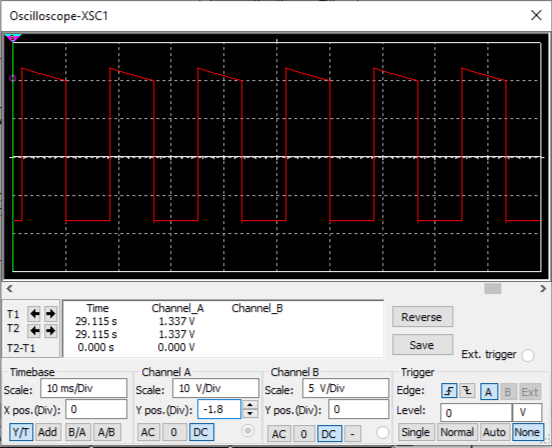
\includegraphics[width=0.975\textwidth]{images/simulacoes/osciloscopio_circuito06.png}
        }}
    \caption{Osciloscópio: Circuito grampeador com fonte em série}
    \vspace{-0.3cm}
    \label{fig:OsciloscopioCircuito06}
\end{figure}
